\section{Analisi}
In questo capitolo verranno analizzati i dati raccolti per elaborare le informazioni che possono rispondere alla domande poste inizialmente (sezione \ref{domande-iniziali}).

Per poter fornire un'immagine del brand più realistica e aggiornata possibile sono stati considerati i dati dell'ultimo anno e sono stati confrontati con quelli dell'anno precedente.

Le informazioni più immediate sono il giudizio degli utenti espresso tramite le stelle; le stelle forniscono un indice approssimativo ma immediato di come il brand viene percepito.

La Corsair ha una votazione media di 4.5 stelle su un massimo di 5. Nella figura \ref{fig:analysis_rating} è mostrata la distribuzione di stelle nelle recensioni.

\begin{figure}[ht]
    \centering
    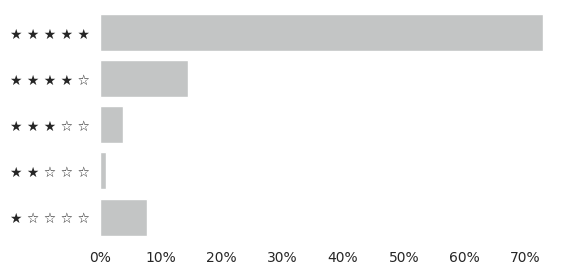
\includegraphics[width=0.85\textwidth]{images/analysis/rating.png}
    \caption{Distribuzione di stelle assegnate alle recensioni di Corsair.}
    \label{fig:analysis_rating}
\end{figure}

Dalle recensioni è possibile capire quali sono i prodotti principali forniti da Corsair, come mostrato nelle figure \ref{fig:analysis_text} e \ref{fig:analysis_text_phrases}. Le principali aree identificate associate al brand sono effettivamente quelle che sappiamo essere relative ai prodotti Corsair. Inoltre si può notare come appaiano parole e frasi che suggeriscono una valutazione del brand positiva, come ``good'', ``great'' e ``i am very happy''.

\begin{figure}[ht]
    \centering
    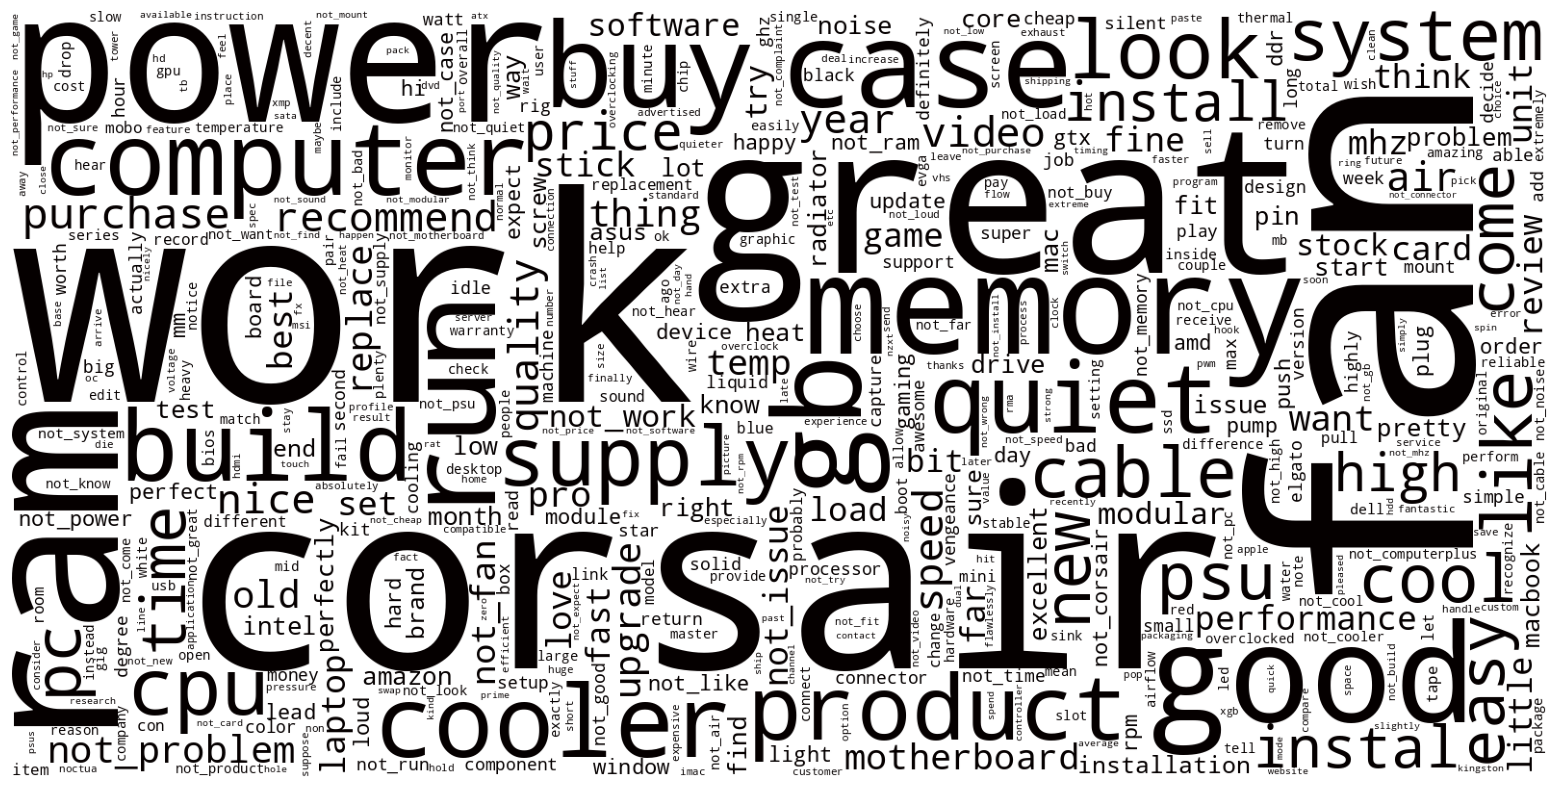
\includegraphics[width=0.85\textwidth]{images/analysis/wc_text.png}
    \caption{Questa wordcloud mostra le parole più ricorrenti all'interno delle recensioni dei prodotti del brand Corsair.}
    \label{fig:analysis_text}
\end{figure}

\begin{figure}[ht]
    \centering
    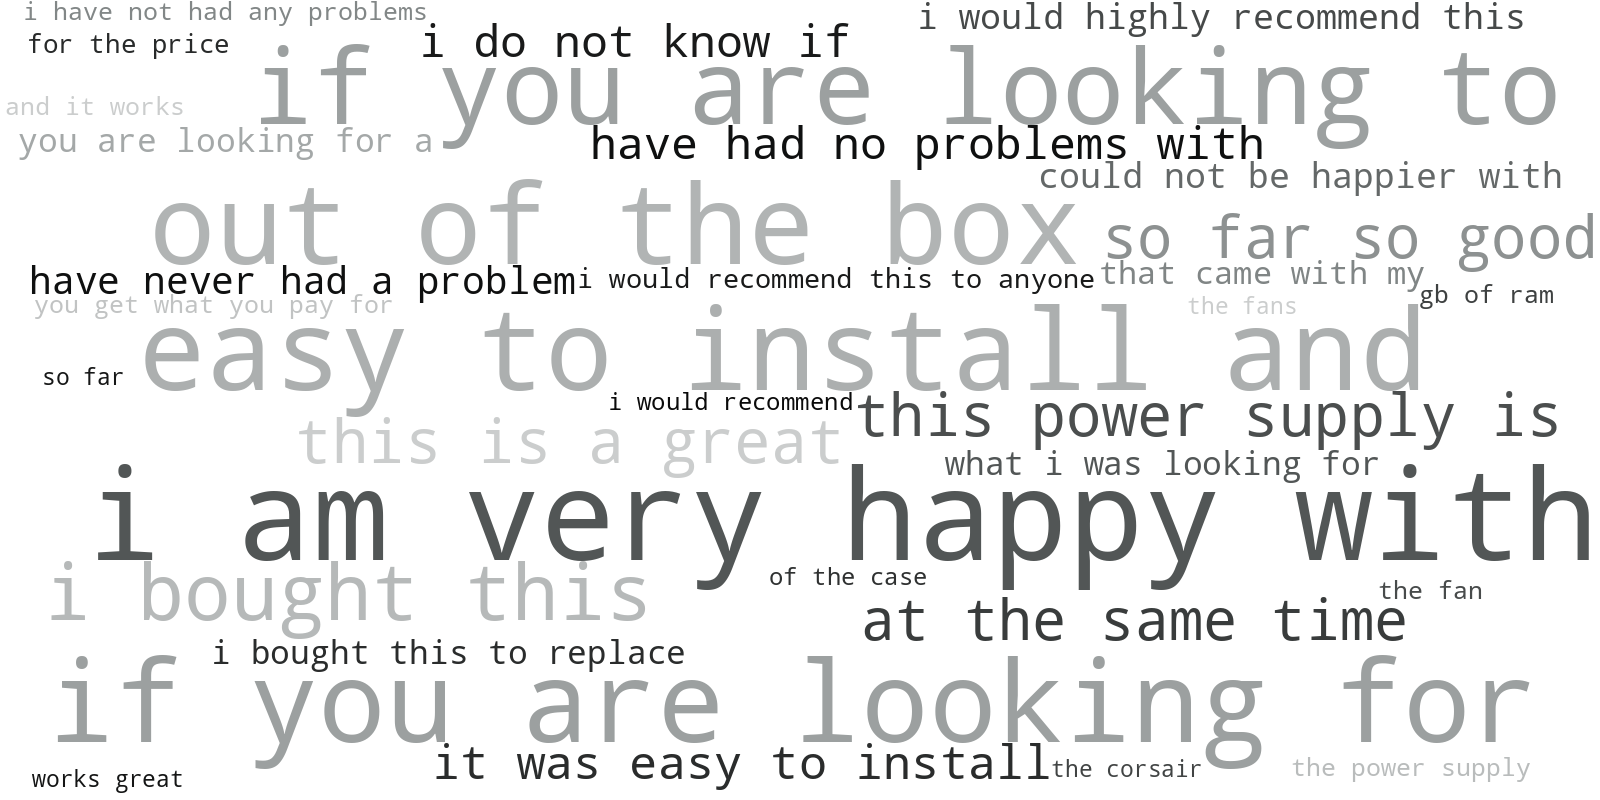
\includegraphics[width=0.9\textwidth]{images/analysis/wc_text_phrases.png}
    \caption{Questa wordcloud mostra le frasi più ricorrenti all'interno delle recensioni dei prodotti del brand Corsair.}
    \label{fig:analysis_text_phrases}
\end{figure}

Per avere informazioni più dettagliate che rispondano alle nostre domande è necessario usare analisi riguardanti gli aspetti e il \textit{sentiment}, le quali permettono di sfruttare le informazioni presenti in ogni singola recensione. 

Dall'analisi delle recensioni emerge che l'82.5\% sono positive, mentre il 17.5\% sono negative. Per andare a valutare in quali recensioni si ha un \textit{sentiment} più negativo è utile analizzare come è distribuito il \textit{sentiment} nelle categorie principali di Corsair.

Nella figura \ref{fig:analysis_category} viene mostrata la distribuzione delle recensioni per categoria
per avere un'idea di quali categorie siano le più recensite dagli utenti. Nella figura \ref{fig:analysis_sentiment_category} viene mostrato il \textit{sentiment} per ogni categoria.

Si può notare come \textit{Memory} e \textit{Fans \& Cooling} siano le categorie di punta del brand, mentre le categoria con \textit{sentiment} più alto risultano \textit{Power Supplies} e \textit{Fans \& Cooling}, seguite da \textit{Memory} e per ultima \textit{TV Tuner \& Capture Cards} che però è quella con meno recensioni.

\begin{figure}[ht]
  \centering
  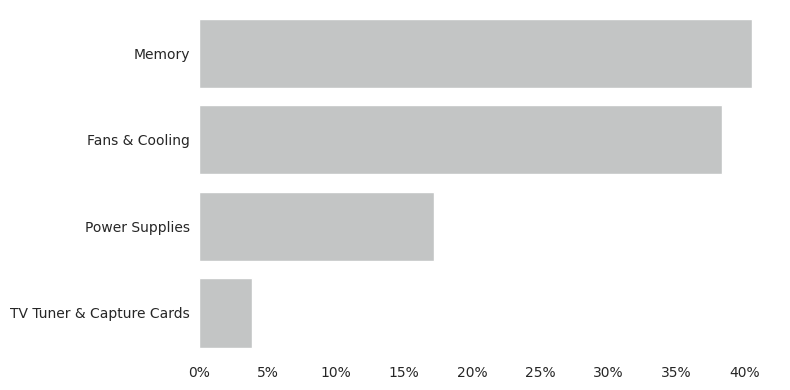
\includegraphics[width=0.95\textwidth]{images/analysis/categories.png}
  \caption{Principali categorie dei prodotti Corsair.}
  \label{fig:analysis_category}
\end{figure}

\begin{figure}[ht]
  \centering
  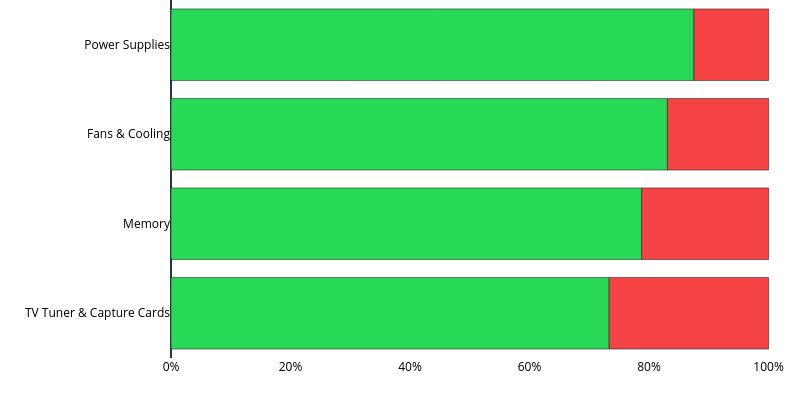
\includegraphics[width=0.95\textwidth]{images/analysis/sentiment_categories.png}
  \caption{\textit{Sentiment} delle principali categorie dei prodotti Corsair.}
  \label{fig:analysis_sentiment_category}
\end{figure}

Un'ulteriore analisi che si può effettuare è quella degli aspetti più menzionati nelle recensioni (figura \ref{fig:analysis_topics}) e come per le categorie, andare a vedere la distribuzione del \textit{sentiment} per ogni aspetto.  
Questo è utile per capire quali aspetti vengono associati al brand dagli utenti e di cosa si parla nelle recensioni.

\begin{figure}[ht]
  \centering
  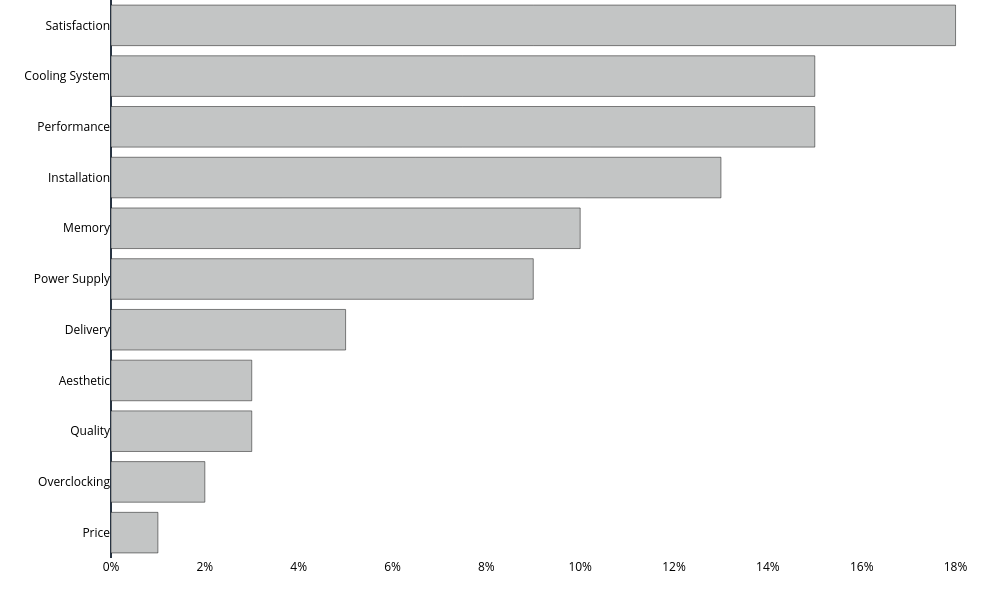
\includegraphics[width=0.95\textwidth]{images/analysis/topics.png}
  \caption{Aspetti più menzionati nelle recensioni.}
  \label{fig:analysis_topics}
\end{figure}

Nella figura \ref{fig:analysis_topics_sentiment} si possono notare gli aspetti di forza del brand come \textit{Aesthetic} e \textit{Power Supply}; in corrispondenza si possono notare gli aspetti valutati in modo più negativo come \textit{Price}, \textit{Overclocking} e \textit{Performance}. 

L'aspetto \textit{Price}, nonostante sia uno dei più negativi è menzionato in poche recensioni (figura \ref{fig:analysis_topics}), al contrario di \textit{Performance} che determina quindi un fattore negativo per il brand.

\begin{figure}[ht]
  \centering
  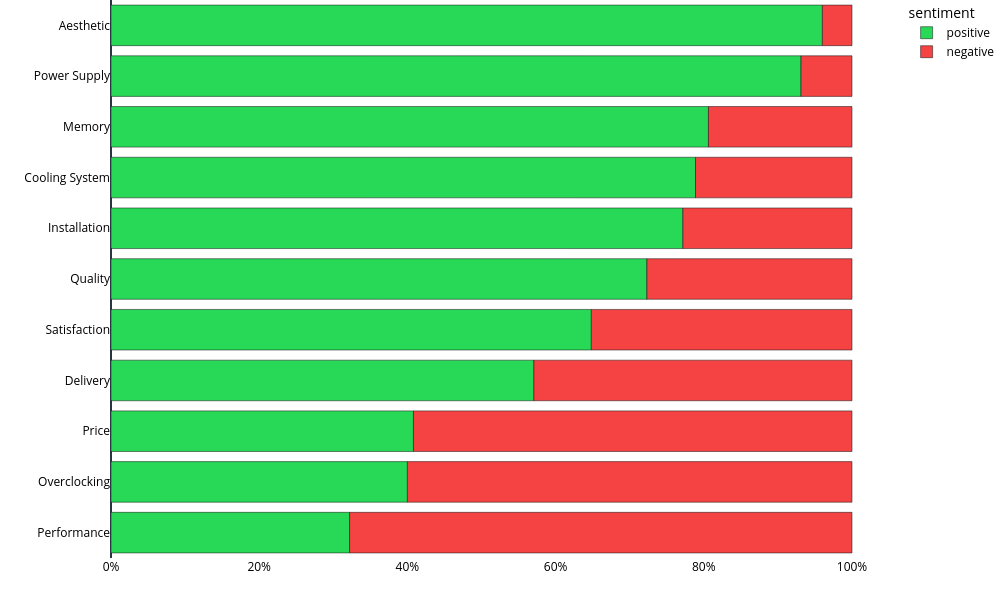
\includegraphics[width=0.95\textwidth]{images/analysis/topics_sentiment.png}
  \caption{Distribuzione del \textit{sentiment} degli aspetti più menzionati nelle recensioni.}
  \label{fig:analysis_topics_sentiment}
\end{figure}

\newpage

Dopo aver effettuato queste analisi il passo successivo è stato individuare i principali competitor del brand Corsair in base alle categorie di prodotti più recensiti per poter effettuare un confronto.
Nelle seguenti figure (\ref{fig:analysis_competitor_memory}, \ref{fig:analysis_competitor_fans}, \ref{fig:analysis_competitor_power} e \ref{fig:analysis_competitor_tv}) viene mostrato il \textit{sentiment} positivo associato a ciascun competitor per ogni categoria.
Dalle figure emerge come tutti i competitor godano di una buona valutazione da parte degli utenti e inoltre le differenze tra i vari brand non sono significative.

\begin{figure}[ht]
  \centering
  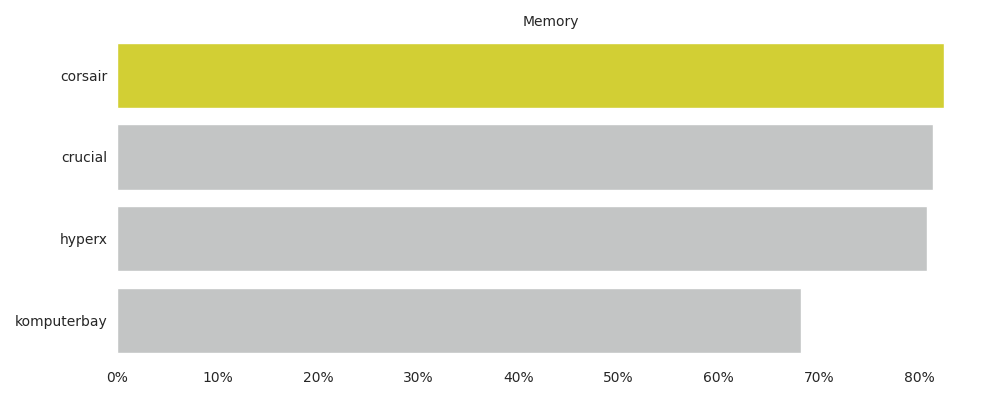
\includegraphics[width=0.95\textwidth]{images/analysis/competitors_Memory.png}
  \caption{\textit{Sentiment} positivo associato ai principali competitor del brand rispetto alla categoria \textit{Memory}.}
  \label{fig:analysis_competitor_memory}
\end{figure}

\begin{figure}[p]
  \centering
  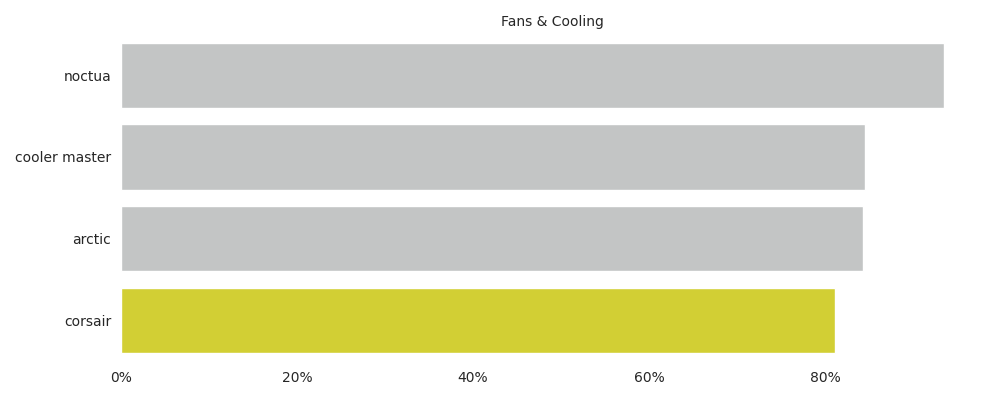
\includegraphics[width=0.95\textwidth]{images/analysis/competitors_Fans & Cooling.png}
  \caption{\textit{Sentiment} positivo associato ai principali competitor del brand rispetto alla categoria \textit{Fans \& Cooling}.}
  \label{fig:analysis_competitor_fans}
\end{figure}

\begin{figure}[p]
  \centering
  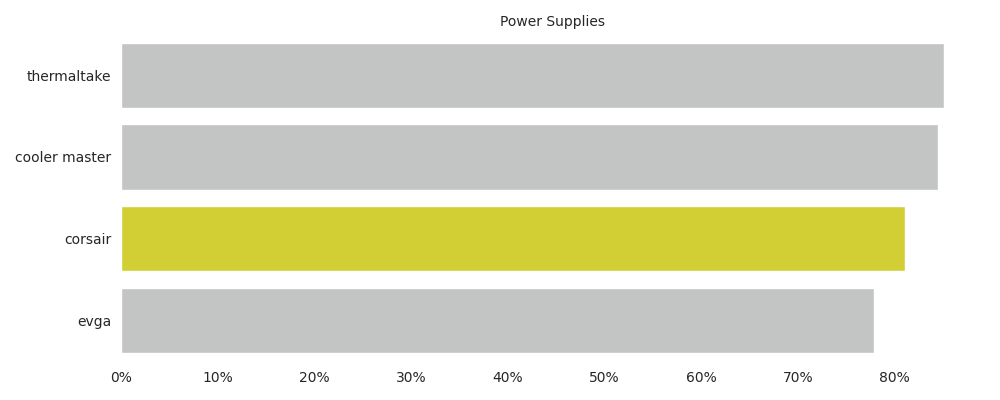
\includegraphics[width=0.95\textwidth]{images/analysis/competitors_Power Supplies.png}
  \caption{\textit{Sentiment} positivo associato ai principali competitor del brand rispetto alla categoria \textit{Power Supplies}.}
  \label{fig:analysis_competitor_power}
\end{figure}

\begin{figure}[p]
  \centering
  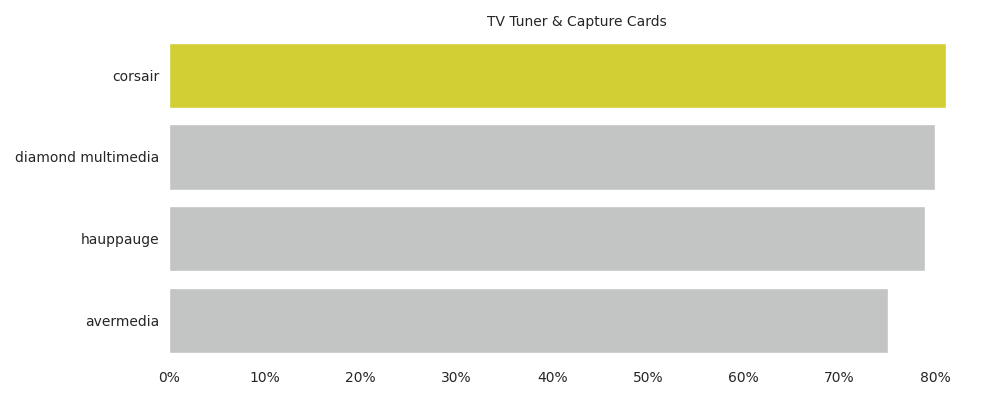
\includegraphics[width=0.95\textwidth]{images/analysis/competitors_TV Tuner & Capture Cards.png}
  \caption{\textit{Sentiment} positivo associato ai principali competitor del brand rispetto alla categoria \textit{TV Tuner \& Capture Cards}.}
  \label{fig:analysis_competitor_tv}
\end{figure}

\newpage 

Nelle figure \ref{fig:analysis_spider_memory} e \ref{fig:analysis_spider_fan} è possibile notare un dettaglio ancora maggiore, in questi grafici viene rappresentato per ogni competitor e per le due categorie \textit{Memory} e \textit{Fans \& Cooling} il \textit{sentiment} positivo per ogni singolo topic.
Questa analisi così dettagliata può permettere di capire quali aspetti possono essere causa di una migliore o peggiore valutazione da parte dell'utente e quindi capire su quali punti il brand dovrebbe focalizzarsi per poter migliorare i propri prodotti.

Nella figura \ref{fig:analysis_spider_memory} si può notare come Corsair e Crucial non solo abbiano una valutazione generale molto simile, ma anche la valutazione sul singolo topic è molto simile, a eccezione del topic \textit{Performace}, che come già notato risulta avere un \textit{sentiment} positivo basso.

\begin{figure}[ht]
  \centering
  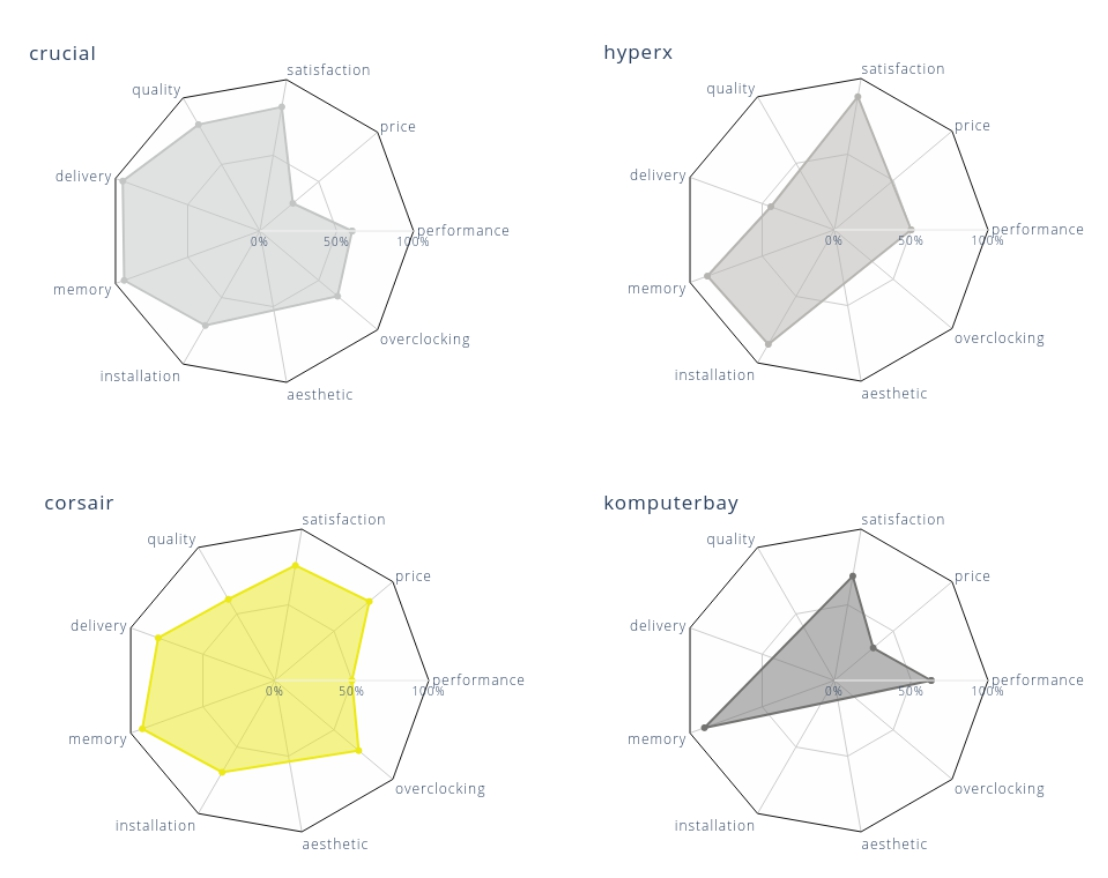
\includegraphics[width=0.95\textwidth]{images/analysis/analysis_memory_spider.jpg}
  \caption{Confronto dei competitor del \textit{sentiment} positivo per ogni singolo topic per la categoria \textit{Memory}.}
  \label{fig:analysis_spider_memory}
\end{figure}

Nella figura \ref{fig:analysis_spider_fan} il valore di \textit{Aesthetic} è molto elevato per Corsair mentre il valore di \textit{Price} è il più basso fra i competitor, questo può indicare come una migliore estetica del prodotto sia apprezzata dagli utenti, ma pesi comunque di più un prezzo più elevato. Di conseguenza si ottiene un abbassamento della valutazione generale e quindi una minor competitività rispetto agli altri brand.

\begin{figure}[ht]
  \centering
  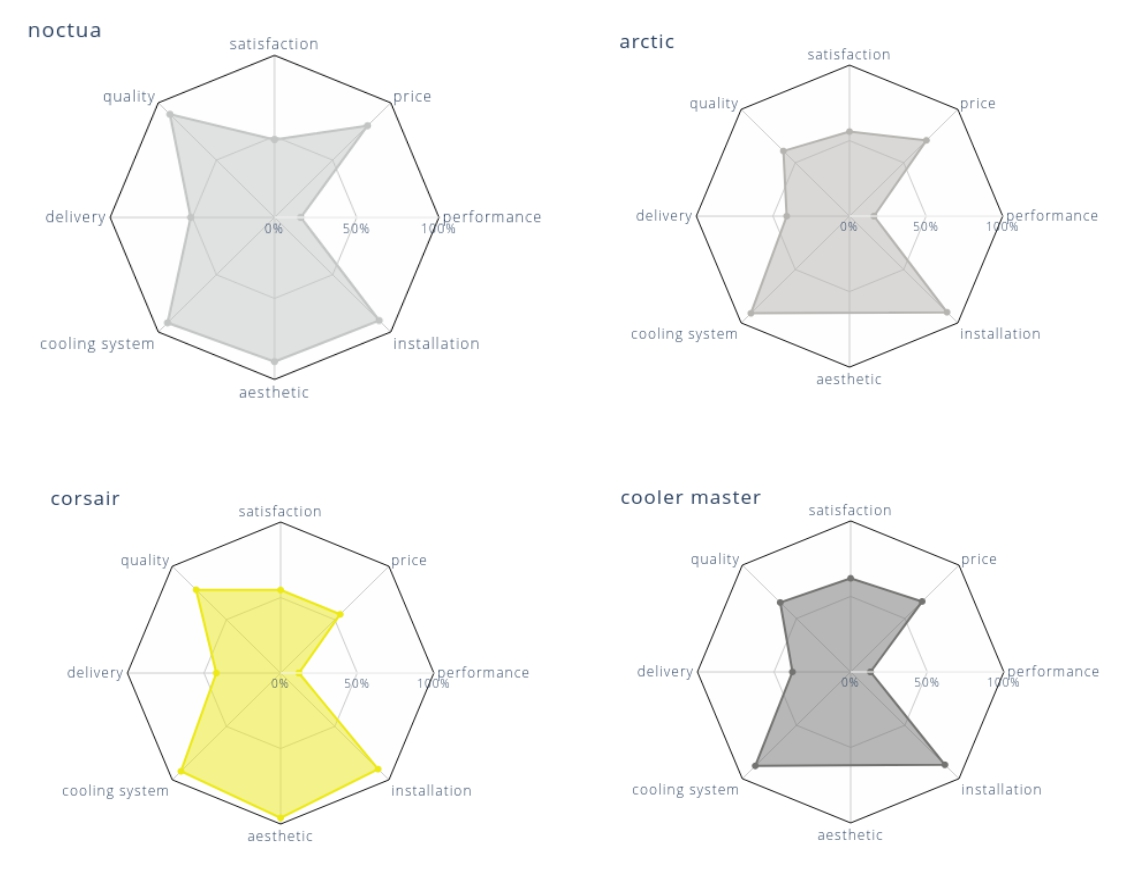
\includegraphics[width=0.95\textwidth]{images/analysis/analysis_fan_spider.jpg}
  \caption{Confronto dei competitor del \textit{sentiment} positivo per ogni singolo \textit{topic} per la categoria \textit{Fans \& Cooling}.}
  \label{fig:analysis_spider_fan}
\end{figure}